\documentclass[aspectratio=169]{beamer}
\usepackage[utf8]{inputenc}
\usepackage[ngerman]{babel}
\usepackage{microtype}
\usepackage{siunitx}
\usepackage{xspace}
\usepackage{tikz}
\usepackage{pgfpages}
\usepackage{pgfplots}
\usepackage{circuitikz}
\usepackage{adjustbox}
\usepackage{textcomp}
\usepackage{minted}
\usepackage{multicol}
\usetikzlibrary{shapes, chains, positioning}
\usepgfplotslibrary{fillbetween}
\useoutertheme{infolines}
\setbeamertemplate{navigation symbols}{}%remove navigation symbols
\usecolortheme[]{solarized}
\colorlet{defaultcolor}{fg}
\mode<handout>{%
    \pgfpagesuselayout{2 on 1}[a4paper] 
    \setbeameroption{show notes}
}
\newcommand{\BPF}[2] 
{  % #1 = name , #2 = rotation angle
\begin{scope}[transform shape,rotate=#2]
\draw[thick] (#1)node[](a){} +(-12pt,-12pt) rectangle +(12pt,12pt);
\draw (a) +(-8pt,0) to[bend left] +(0,0) edge[bend right] +(8pt,0);
\draw ([yshift=5pt]a) +(-8pt,0) to[bend left] +(0,0) to[bend right] +(8pt,0);
\draw ([yshift=-5pt]a) +(-8pt,0) to[bend left] +(0,0) edge[bend right] +(8pt,0);
\draw[rotate=20] ([yshift=5pt]a) +(-4pt,0) -- +(7pt,0);
\draw[rotate=20] ([yshift=-5pt]a) +(-7pt,0) -- +(4pt,0);
\end{scope}
}
%
\newcommand{\GR}{GNU\,Radio}
\titlegraphic{\centering%

\includegraphics[width=\paperwidth,bb={109 0 1069 200}]{sdr-titlepage.pdf}%
}
%\logo{\includegraphics[width=\paperwidth,bb={109 0 1069 200}]{sdr-logo.pdf}}
\logo{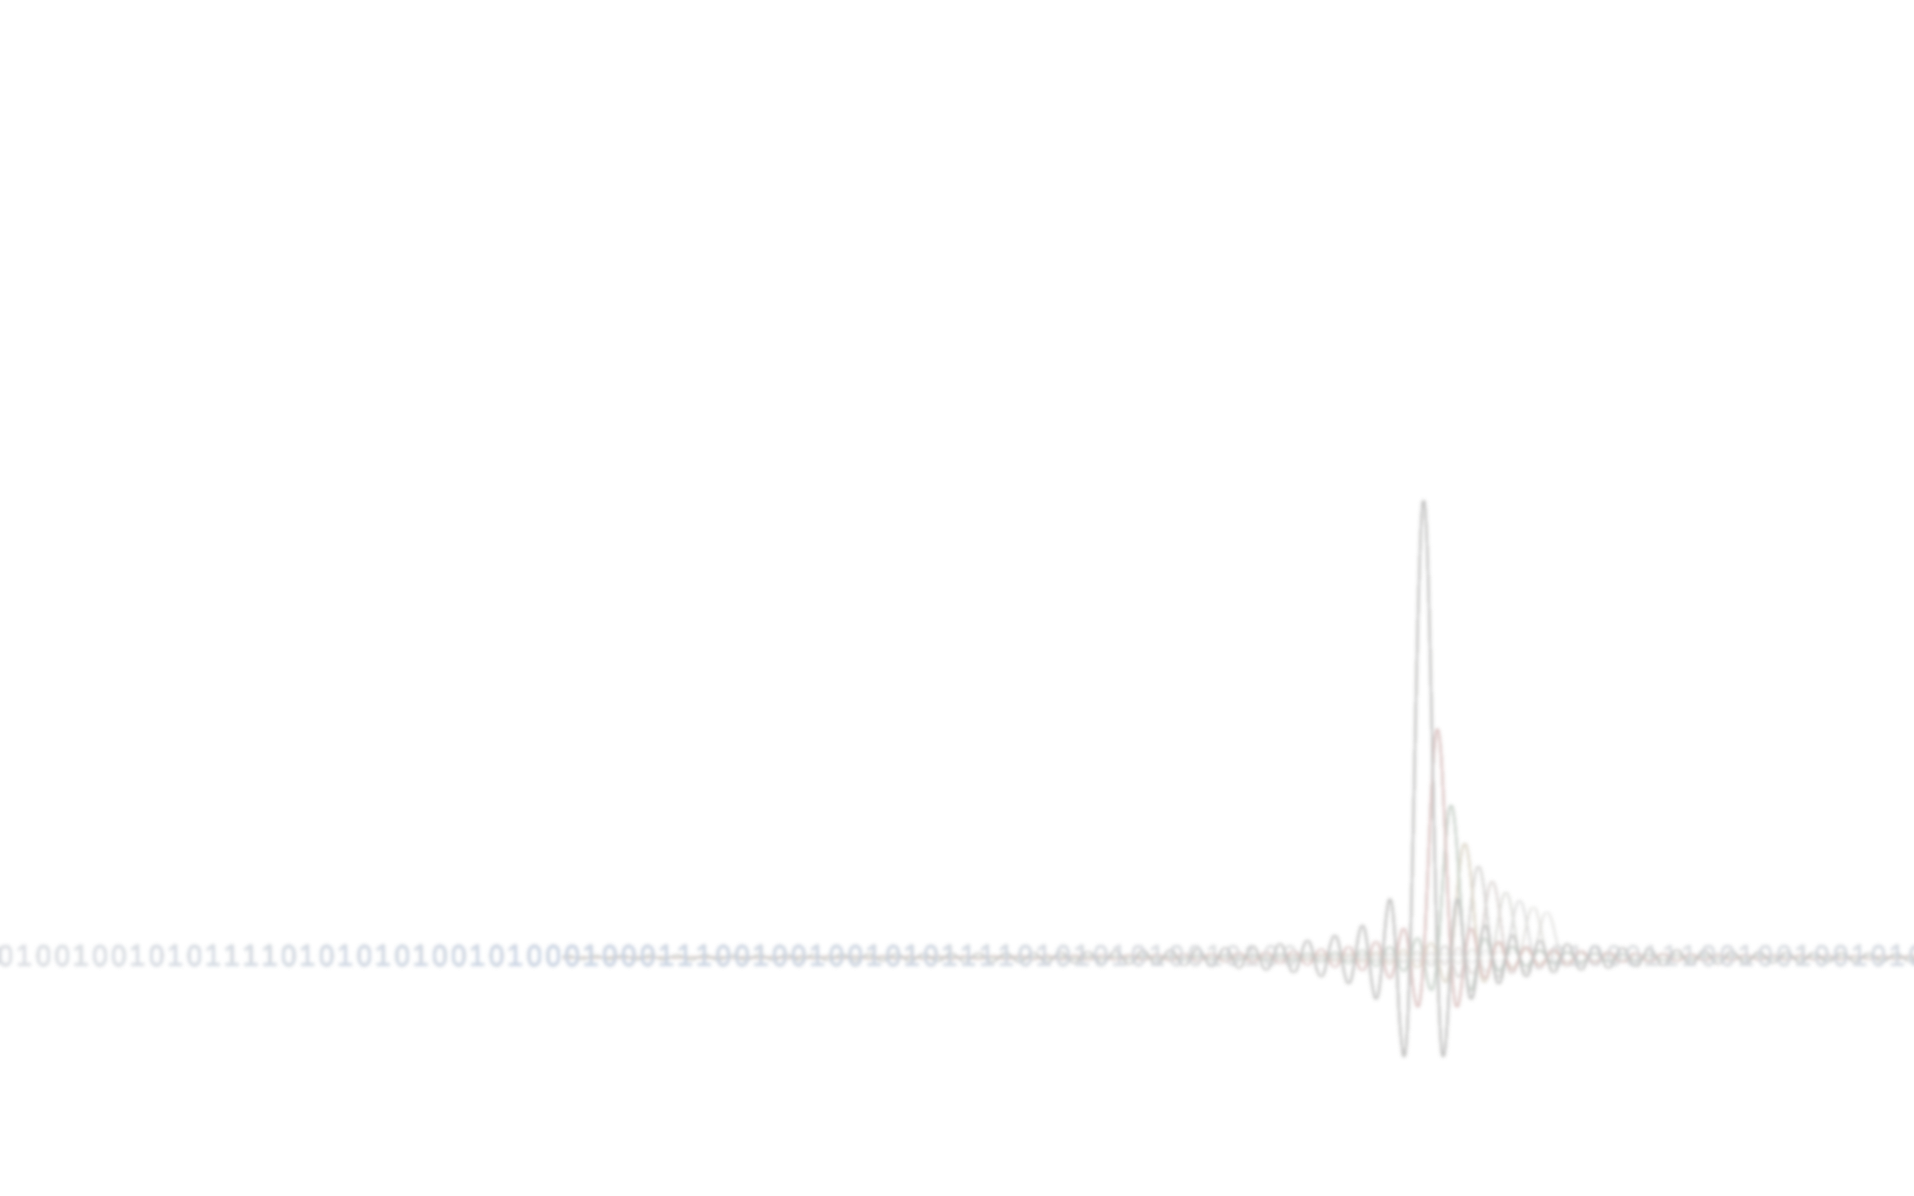
\includegraphics[width=\paperwidth]{sdr-logo-1920.png}}
\date{2023-06-01 23:32}
\title{SigMF Introduction}
\author{Marcus Müller}
%\institute{Marcus Müller Engineering}

\begin{document}
\frame[plain]{\titlepage}
\begin{frame}{Table of Contents}
  \tableofcontents
\end{frame}

\section{SigMF in 25\,s}
\begin{frame}{}\frametitle{SigMF in 25\,s}
  \hfill
\includegraphics[width=0.2\textwidth,keepaspectratio]{sigmf_logo.png}

  \vspace{-0.15\textwidth}
  SigMF:
  \begin{itemize}
    \item Metadata Specification (mostly) for time signal data
    \item Designed by a community mostly concerned with radio signals
    \item JSON-based format with clear spec that defines, unambiguously
      \begin{itemize}
        \item  data types\\([un]signed integer, \{single,double\} precision float, endianness, complex of these, \ldots)
        \item  interpretation (time signal, spectra, …)
        \item  ensembles of recordings
        \item \textbf<2>{position, scope and length of annotations}
      \end{itemize}
    \item Tooling and Community around the spec
  \end{itemize}
\end{frame}

\section{Original Problem Field}
\begin{frame}{Original Problem Field}
  SDR -- Software Defined Radio: Processing / producing radio signals in software\\(rather than hardware)
  \begin{itemize}
    \item ``Soundcard on Speed'': For a couple kHz sound bandwidth, sampling at 48\,kHz sufficient\\
      Radio signals have bandwidths in MHz $\rightarrow$ SDRs sample in MHz
      \begin{itemize}
        \item Very little / no room for overhead when streaming to disk
      \end{itemize}
    \item Signal-to-disk common requirement
      \begin{itemize}
        \item Radio astronomy
        \item Transmitter/Receiver development
        \item Spectrum surveillance
        \item Training of neural networks
        \item Increasingly popular among physicist (GSI Darmstadt/FAIR)
      \end{itemize}
    \item Signal often bursty, always noisy
    \item \textbf<2>{Desirable to mark relevant segments}
  \end{itemize}
\end{frame}

\subsection{History / Provenance}
\begin{frame}{History / Provenance}
  \begin{itemize}
    \item GNU\,Radio: Dominant SDR framework for processing
      \begin{itemize}
        \item Free \& Open Source $\rightarrow$ relevant for US national-level radio research community
        \item Performant enough to enable running software on standard laptop-style computers
      \end{itemize}
    \item DARPA sponsors an SDR hackfest 2017 in Brussels\\
      (heavy GNU Radio involvement, but \emph{not} a GR hackfest)
    \item Result: Draft of a universally useful metadata format for radio data
    \item Since then: Community improvement process, stable spec \url{https://github.com/sigmf/SigMF}
  \end{itemize}
\end{frame}

\section{SigMF in Practice}
\begin{frame}{SigMF in Practice}
  \begin{itemize}
    \item JSON format specification
    \item Separate file or in uncompressed archive (tar) alongside capture data files\\[2em]

    \item Metadata encompasses
      \begin{itemize}
        \item Data type information
        \item Whole-Capture metadata (human description, time, rate, setup information, \# channels, \ldots)
        \item List of captures
        \item \textbf{List of Annotations}
      \end{itemize}
  \end{itemize}
\end{frame}

\subsection{Example}
\begin{frame}{Example -- IQEngine view}
  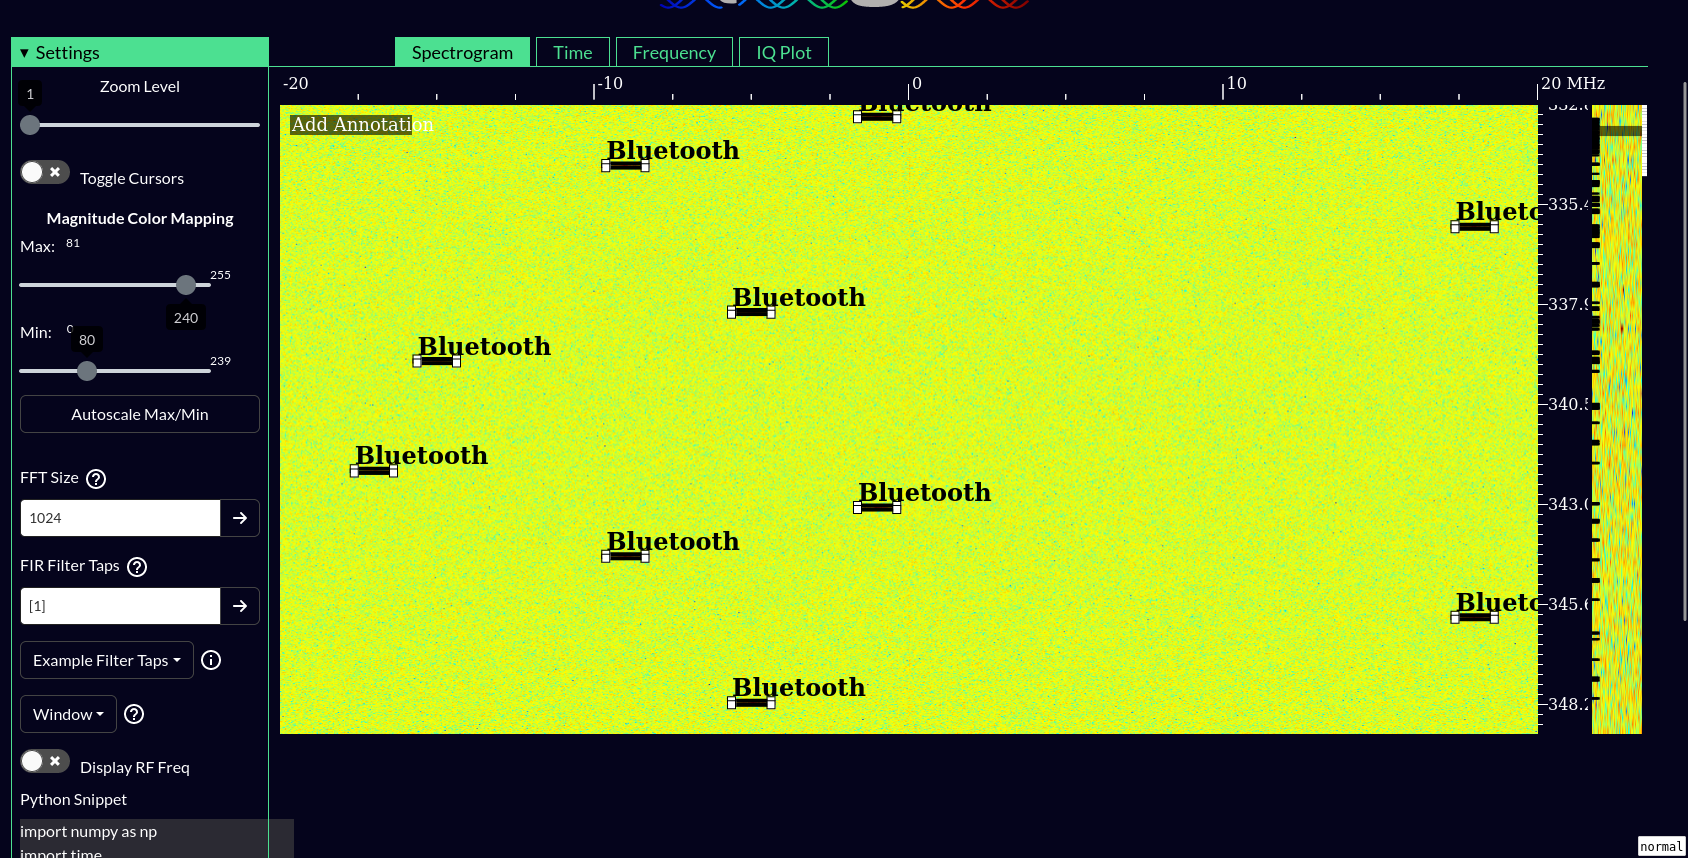
\includegraphics[width=\textwidth,keepaspectratio]{screen.png}
\end{frame}

\begin{frame}{\quad Example -- SigMF Metadata}
  \vspace{-1.5em}
  \begin{columns}
    \begin{column}{0.48\textwidth}
  \scriptsize\inputminted[lastline=24]{json}{meta.json}
  \end{column}
    \begin{column}{0.48\textwidth}
  \scriptsize\inputminted[firstline=25,lastline=48]{json}{meta.json}
  \end{column}
  \end{columns}
\end{frame}

\section{Extensibility}
\begin{frame}{SigMF Extensibility}
 SigMF supports \emph{extension namespaces}:

While canonical specification desirable, allowing users to well-define own namespace critical

Namespaces definition itself specified
\end{frame}


\section*{Q\&A}
\begin{frame}{Questions?}
  
\end{frame}

\end{document}
